\documentclass[conference]{IEEEtran}
\IEEEoverridecommandlockouts

% ================= PACKAGES =================
\usepackage{cite}
\usepackage{amsmath,amssymb,amsfonts}
\usepackage{algorithmic}
\usepackage{graphicx}
\usepackage[utf8]{inputenc}
\usepackage{textgreek}
\usepackage{textcomp} % For symbols like \textdegree and \textmu
\usepackage{xcolor}
\usepackage{listings}
\usepackage{caption}
\usepackage{subcaption}
\usepackage{booktabs} % For professional tables
\usepackage{multirow}
\usepackage{array}
\usepackage{float}
\usepackage{siunitx} % For proper unit formatting

% Bibliography formatting
\def\BibTeX{{\rm B\kern-.05em{\sc i\kern-.025em b}\kern-.08em
    T\kern-.1667em\lower.7ex\hbox{E}\kern-.125emX}}

\begin{document}

% ================= TITLE =================
\title{Design and Analysis of Two MOS Differential Amplifier Topologies: A Comparative Study}

% ================= AUTHORS =================
\author{
\IEEEauthorblockN{Siddhant Shah (B23334)\textsuperscript{*}, 
                  Aman (T25121)\textsuperscript{†}, 
                  Omkar Sharan (T25132)\textsuperscript{‡}}
\IEEEauthorblockA{\textsuperscript{*}b23334@students.iitmandi.ac.in \\
                  \textsuperscript{†}t25121@students.iitmandi.ac.in \\
                  \textsuperscript{‡}t25132@students.iitmandi.ac.in}
}

\maketitle

% ================= ABSTRACT =================
\begin{abstract}
\noindent
This report presents a comprehensive comparative analysis of two CMOS differential amplifier topologies: one with NMOS as the tail current source and another with PMOS as the tail current source. The performance of each circuit is characterized through simulation, focusing on key metrics including small-signal differential gain, phase margin, unity-gain bandwidth (UGBW), and average power dissipation. For the NMOS-tail amplifier, measured results show: differential gain = 28.5717 dB, UGBW = 3.081 MHz, phase margin = 87.83\textdegree, and average power = 3.635~\textmu W. The PMOS-tail amplifier demonstrates: differential gain = 32.2347 dB, UGBW = 2.134 GHz, phase margin = 76.54\textdegree, and average power = 3.032~\textmu W. This study highlights the fundamental design trade-offs between different tail current implementations in terms of performance, stability, power efficiency, and the critical impact of device sizing on bandwidth characteristics.
\end{abstract}

% ================= KEYWORDS =================
\begin{IEEEkeywords}
MOS Differential Amplifier, Differential Gain, Unity-Gain Bandwidth (UGBW), Phase Margin, CMOS Analog Circuits, Active Load, Current Mirror, Biasing, Tail Current Source
\end{IEEEkeywords}

% ================= INTRODUCTION =================
\section{Introduction}
\noindent
Differential amplifiers represent a cornerstone of modern analog integrated circuit (IC) design, serving as the primary front-end stage in systems requiring high signal integrity. Their fundamental strength lies in amplifying the difference between two input signals while simultaneously rejecting common-mode noise—a critical capability in noisy mixed-signal environments \cite{razavi}. This inherent common-mode rejection ratio (CMRR) makes differential amplifiers essential building blocks in operational amplifiers, comparators, analog-to-digital converters, and sensor interface circuits \cite{gray, johns}.

\noindent
This work presents the detailed analysis and comparison of two practical MOS differential amplifier topologies implemented in CMOS technology. The first design utilizes a conventional NMOS transistor to form the tail current source, which is the most common configuration in modern analog design \cite{razavi}. The second topology investigates the use of a PMOS transistor for the tail current source, offering a different set of performance trade-offs, particularly in relation to common-mode input range, noise characteristics, and input pair transconductance \cite{allen, baker}. Both topologies feature single-ended outputs and active loads to achieve high voltage gain without the silicon area penalty of resistive loads \cite{gray}.

\noindent
The choice between NMOS and PMOS tail current sources has significant implications for circuit performance. NMOS-tail amplifiers typically offer higher input common-mode range when operating near ground, while PMOS-tail designs can provide advantages in terms of flicker noise and are often preferred when the input common-mode voltage is near the supply rail \cite{johns}. Additionally, the fundamental differences in carrier mobility between NMOS and PMOS devices directly impact the transconductance of the input differential pair, which governs both gain and bandwidth \cite{razavi}.

\noindent
The core of this analysis focuses on quantifying and comparing the key performance metrics for both amplifiers: \textbf{differential gain}, \textbf{unity-gain bandwidth (UGBW)}, \textbf{phase margin (PM)}, and \textbf{power dissipation}. These metrics are intrinsically linked, governed by the fundamental trade-offs between gain, speed, stability, and power consumption that define analog design \cite{allen, carusone}. Using AC and transient simulation measurements, this paper evaluates each amplifier's performance and provides insights into the design considerations for selecting the appropriate topology for specific applications.

% ================= DESIGN SPECIFICATIONS =================
\section{Design Specifications}
\noindent
The target specifications for both amplifier designs were based on typical requirements for operational amplifier input stages and analog front-end circuits \cite{razavi, gray}. These expected values are summarized in Table~\ref{tab:specs}. The specifications emphasize high gain, moderate bandwidth, excellent stability, and low power consumption—characteristics typical of low-power analog signal processing applications.

\begin{table}[H]
    \centering
    \caption{Target Design Specifications for Both Amplifiers}
    \label{tab:specs}
    \begin{tabular}{@{}ll@{}}
        \toprule
        \textbf{Parameter} & \textbf{Expected/Design Value} \\
        \midrule
        Differential Gain (dB) & 50 \\
        UGBW (MHz) & 100 \\
        Phase Margin (\textdegree) & $\geq$ 60 (target: 90) \\
        Power (\textmu W) & Minimize \\
        \bottomrule
    \end{tabular}
\end{table}

% ================= QUESTION 1 =================
\section{NMOS-Tail Differential Amplifier}

\subsection{Circuit Description}
\noindent
The amplifier circuit, shown in Fig.~\ref{fig:nmos_tail_diff_amp}, is a five-transistor differential amplifier with NMOS input pair. This circuit uses ideal DC voltage sources for biasing instead of a more complex external bias generator circuit, simplifying the analysis and focusing attention on the core differential amplifier performance \cite{razavi}.

\begin{figure}[H]
    \centering
    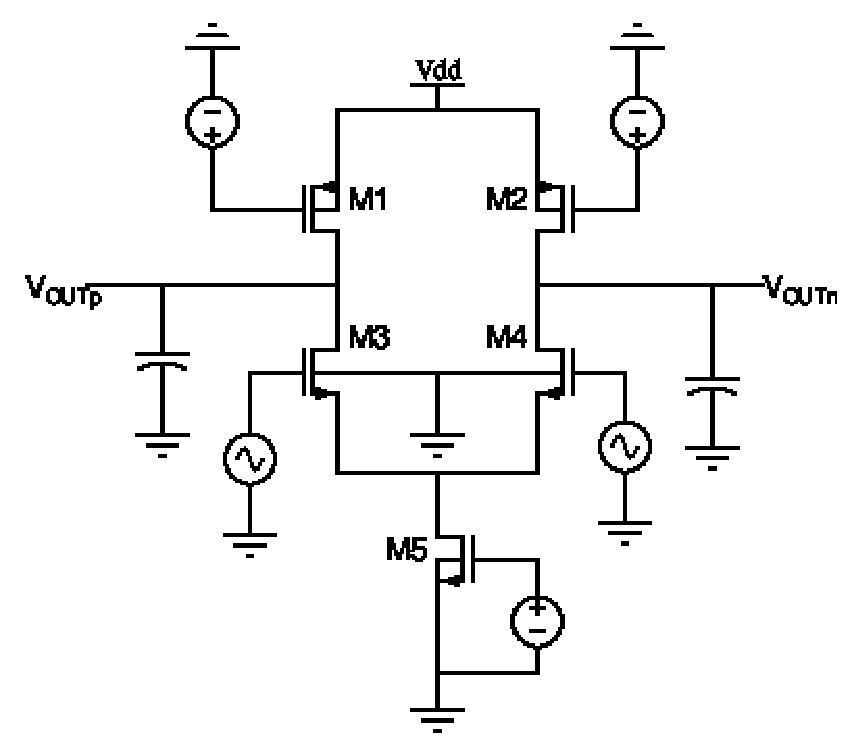
\includegraphics[width=0.5\textwidth]{LAB_5_CKT_1.eps}
    \caption{NMOS-tail differential amplifier with ideal bias sources.}
    \label{fig:nmos_tail_diff_amp}
\end{figure}

The main functional blocks are:
\begin{itemize}
    \item \textbf{Input differential pair (M3, M4):} These NMOS transistors convert the differential input voltage $v_{id}$ (applied to their gates) into differential currents. Operating in saturation, they provide the transconductance ($g_m$) that primarily determines the amplifier's gain. The transconductance is given by $g_m = \sqrt{2\mu_n C_{ox} (W/L) I_D}$ for NMOS devices in saturation \cite{razavi}.
    
    \item \textbf{Active PMOS loads (M1, M2):} These PMOS transistors act as active loads, functioning as high-value resistors. Their gates are biased by independent ideal DC voltage sources (1.2 V) to establish the output common-mode level and provide a high output resistance ($r_o$) for increased differential gain. The voltage gain is approximately $A_d = g_{m,M3} (r_{o,M2} \parallel r_{o,M4})$ \cite{gray, allen}.
    
    \item \textbf{NMOS tail current source (M5):} This NMOS transistor, biased by an ideal DC voltage source (540 mV), provides a constant bias current ($I_{SS}$) to the input pair. This tail current source is essential for achieving high common-mode rejection ratio (CMRR), as it ideally presents infinite impedance to common-mode signals \cite{allen, johns}.
    
    \item \textbf{Load capacitors ($C_L$):} The 1~pF capacitors represent the parasitic or explicit load capacitance at the output nodes. This capacitance, along with the output resistance, determines the dominant pole location and hence the bandwidth of the amplifier. The dominant pole frequency is approximately $f_p = 1/(2\pi R_{out} C_L)$ \cite{carusone}.
\end{itemize}

\subsection{Component Specifications}
\noindent
The device parameters and simulation sources used for this analysis are detailed in Table~\ref{tab:transistors_q1} and Table~\ref{tab:sources_q1}. Note that all transistors use relatively long channel lengths (L = 0.54 \textmu m), which increases output resistance and improves gain at the expense of transconductance \cite{baker}.

\begin{table}[H]
    \centering
    \caption{Transistor Sizing (Circuit 1 --- NMOS Tail)}
    \label{tab:transistors_q1}
    \begin{tabular}{@{}lcccc@{}}
        \toprule
        \textbf{Device} & \textbf{Type} & \textbf{W (\textmu m)} & \textbf{L (\textmu m)} & \textbf{Multiplier (m)} \\
        \midrule
        M1 & PMOS & 0.42 & 0.54 & 1 \\
        M2 & PMOS & 0.42 & 0.54 & 1 \\
        M3 & NMOS & 0.42 & 0.54 & 1 \\
        M4 & NMOS & 0.42 & 0.54 & 1 \\
        M5 & NMOS & 0.42 & 0.54 & 1 \\
        \bottomrule
    \end{tabular}
\end{table}

\begin{table}[H]
    \centering
    \caption{Source and Supply Parameters (Circuit 1)}
    \label{tab:sources_q1}
    \begin{tabular}{@{}ll@{}}
        \toprule
        \textbf{Component} & \textbf{Value / Parameters} \\
        \midrule
        Supply Voltage ($V_{DD}$) & 1.8 V \\
        Load Capacitors ($C_L$) & 1 pF \\ 
        PMOS Load Bias (Gates M1, M2) & 1.2 V \\
        NMOS Tail Bias (Gate M5) & 540 mV \\
        \midrule
        \multicolumn{2}{@{}l@{}}{\textbf{Input Source 1 (Gate M3)}} \\
        \quad DC Bias & 600 mV \\
        \quad AC Magnitude & 500 mV \\
        \quad Transient Amplitude & 100 \textmu V \\
        \quad Phase & 180\textdegree \\
        \quad Frequency & 1 GHz \\ 
        \midrule
        \multicolumn{2}{@{}l@{}}{\textbf{Input Source 2 (Gate M4)}} \\
        \quad DC Bias & 600 mV \\
        \quad AC Magnitude & $-$500 mV \\
        \quad Transient Amplitude & 100 \textmu V \\
        \quad Phase & 0\textdegree \\
        \quad Frequency & 1 GHz \\
        \bottomrule
    \end{tabular}
\end{table}

\subsection{Results and Observations}
\noindent
The following performance metrics were obtained from AC and transient simulation measurements for Circuit 1:

\begin{itemize}
    \item Measured differential gain: $A_{d,dB}$ = 28.5717 dB (linear gain $\approx$ 26.9)
    \item Measured unity-gain frequency: $f_{UGBW}$ = 3.081 MHz
    \item Measured phase margin: PM = 87.83\textdegree
    \item Measured average power dissipation: $P_{avg}$ = 3.635 \textmu W
\end{itemize}

\subsubsection{Frequency Response Analysis}
\noindent
The amplifier's frequency response is shown in Fig.~\ref{fig:nmos_tail_bode}, which displays both the magnitude and phase characteristics of the differential gain. The plot clearly shows a single-pole roll-off characteristic, typical of simple differential amplifier topologies \cite{razavi}.

\begin{figure}[H]
    \centering
    \includegraphics[width=0.4\textwidth]{lab_5_ckt_1_bode_plot.png}
    \caption{Gain and phase vs. frequency Bode plot (Circuit 1).}
    \label{fig:nmos_tail_bode}
\end{figure}

\subsubsection{Transient Analysis}
\noindent
The transient response, shown in Fig.~\ref{fig:nmos_tail_transient}, was simulated to observe the amplifier's behavior with a differential step input. This helps visualize the settling time and any ringing, which is expected to be minimal given the high phase margin.

\begin{figure}[H]
    \centering
    % Placeholder for your transient plot
    \includegraphics[width=0.45\textwidth]{lab_5_ckt_1_tran.png}
    \caption{Transient response.}
    \label{fig:nmos_tail_transient}
\end{figure}

\subsubsection{Performance Analysis}
\noindent
The measured results for the NMOS-tail amplifier show significant deviations from the design targets, particularly in gain and bandwidth. This analysis examines the fundamental reasons for these deviations.

\begin{itemize}
    \item \textbf{Gain:} The achieved differential gain of 28.57 dB is well below the 50 dB target. This deficit can be attributed to the product of transconductance ($g_m$) of the input pair (M3, M4) and the total output resistance ($R_{out} = r_{o,M2} \parallel r_{o,M4}$) being lower than required. Given the very small device dimensions (W/L = 0.42/0.54 $\approx$ 0.78) and low bias current, both $g_m$ and $r_o$ are compromised \cite{razavi, allen}.
    
    \item \textbf{Bandwidth:} The unity-gain bandwidth of 3.081 MHz is far short of the 100 MHz target. The UGBW is given by the relationship:
    \begin{equation}
    UGBW = \frac{g_m}{2\pi C_L}
    \end{equation}
    Given the 1 pF load capacitance, this measured UGBW corresponds to an input pair transconductance of approximately $g_m \approx 19.3$ \textmu S, which is very low. This directly reflects the extremely low bias current used in this ultra-low-power design \cite{carusone}.
    
    \item \textbf{Power and Trade-offs:} The low $g_m$ is a direct consequence of the minimal power budget. The average power dissipation of 3.635 \textmu W is exceptionally low, corresponding to a total supply current of approximately 2.02 \textmu A. This ultra-low quiescent current severely limits the transconductance of M3/M4, since $g_m \propto \sqrt{I_D}$ \cite{razavi}. This fundamental relationship simultaneously constrains both the DC gain ($A_d = g_m R_{out}$) and the bandwidth ($UGBW \propto g_m$), demonstrating the classic gain-bandwidth-power trade-off in analog design \cite{johns}.
    
    \item \textbf{Stability:} The amplifier exhibits excellent stability with a phase margin of 87.83\textdegree, very close to the ideal 90\textdegree target. This indicates a clean single-pole frequency response with minimal second-order effects and confirms that the amplifier will have negligible overshoot and ringing in its transient response \cite{gray}. The high phase margin is typical of simple, single-stage amplifiers with dominant-pole compensation \cite{carusone}.
    
    \item \textbf{Gain-Bandwidth Product:} The gain-bandwidth product (GBW = $A_{d,linear} \times$ BW) for this circuit is approximately 82.8 MHz, which is less than the target UGBW of 100 MHz. This confirms that the circuit's fundamental $g_m/C_L$ ratio is insufficient to meet the bandwidth specification \cite{razavi}.
\end{itemize}

\noindent
In summary, Circuit 1 demonstrates a classic analog design trade-off: the circuit achieves excellent stability and extremely low power consumption, but at the direct expense of gain and bandwidth. To meet the target specifications, the bias current would need to be increased significantly, which would proportionally increase both $g_m$ and power dissipation \cite{allen}.

% ================= QUESTION 2 =================
\section{PMOS-Tail Differential Amplifier}

\subsection{Circuit Description}
\noindent
The second circuit topology, shown in Fig.~\ref{fig:pmos_tail_diff_amp}, is a differential amplifier that utilizes a PMOS transistor (M5) as the tail current source. This complementary configuration is often explored for applications requiring input common-mode voltages near the positive supply rail, or for exploiting the typically lower flicker noise of PMOS devices \cite{johns, baker}.

\begin{figure}[H]
    \centering
    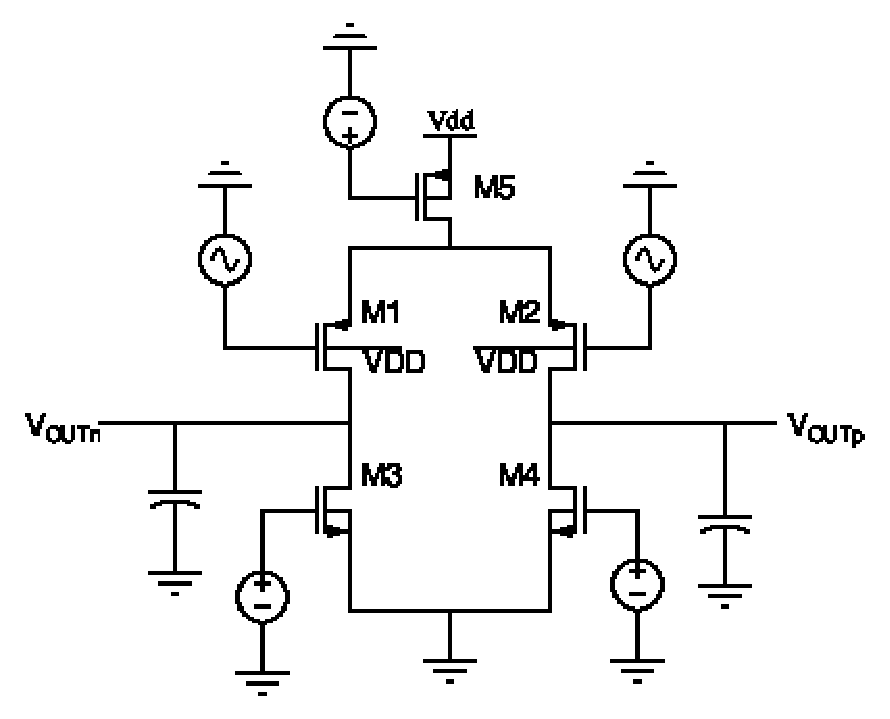
\includegraphics[width=0.5\textwidth]{LAB_5_CKT_2.eps}
    \caption{PMOS-tail differential amplifier with ideal bias sources.}
    \label{fig:pmos_tail_diff_amp}
\end{figure}

The main functional blocks are:
\begin{itemize}
    \item \textbf{Input differential pair (M1, M2):} These PMOS transistors serve as the input transconductance stage, converting the differential input voltage $v_{id}$ into differential currents. The transconductance is given by $g_m = \sqrt{2\mu_p C_{ox} (W/L) I_D}$ for PMOS devices. Note that $\mu_p \approx \mu_n/3$ in typical CMOS processes, which generally results in lower transconductance for PMOS devices at the same geometry and bias current \cite{razavi, gray}.
    
    \item \textbf{Active NMOS loads (M3, M4):} These NMOS transistors act as active loads, providing high output resistance. Their gates are biased by independent ideal DC voltage sources (490 mV) to establish the proper operating point and maximize the differential gain \cite{allen}.
    
    \item \textbf{PMOS tail current source (M5):} This PMOS transistor, biased by an ideal DC voltage source (1.2 V) and connected to $V_{DD}$, provides the constant bias current to the PMOS input pair. The tail current source ensures high CMRR by ideally presenting infinite impedance to common-mode signals \cite{johns}.
    
    \item \textbf{Load capacitors ($C_L$):} The 1~pF capacitors represent the load capacitance at the output nodes, determining the dominant pole and bandwidth characteristics \cite{carusone}.
\end{itemize}

\subsection{Component Specifications}
\noindent
The device parameters and simulation sources are detailed in Table~\ref{tab:transistors_q2} and Table~\ref{tab:sources_q2}. Critically, note that the PMOS input pair (M1, M2) uses a much shorter channel length (L = 0.18 \textmu m) compared to Circuit 1, which dramatically increases transconductance at the expense of output resistance \cite{baker}.

\begin{table}[H]
    \centering
    \caption{Transistor Sizing (Circuit 2 --- PMOS Tail)}
    \label{tab:transistors_q2}
    \begin{tabular}{@{}lcccc@{}}
        \toprule
        \textbf{Device} & \textbf{Type} & \textbf{W (\textmu m)} & \textbf{L (\textmu m)} & \textbf{Multiplier (m)} \\
        \midrule
        M1 & PMOS & 0.42 & 0.18 & 1 \\
        M2 & PMOS & 0.42 & 0.18 & 1 \\
        M3 & NMOS & 0.42 & 0.54 & 1 \\
        M4 & NMOS & 0.42 & 0.54 & 1 \\
        M5 & PMOS & 0.42 & 0.54 & 2 \\
        \bottomrule
    \end{tabular}
\end{table}

\begin{table}[H]
    \centering
    \caption{Source and Supply Parameters (Circuit 2)}
    \label{tab:sources_q2}
    \begin{tabular}{@{}ll@{}}
        \toprule
        \textbf{Component} & \textbf{Value / Parameters} \\
        \midrule
        Supply Voltage ($V_{DD}$) & 1.8 V \\
        Load Capacitors ($C_L$) & 1 pF \\ 
        NMOS Load Bias (Gates M3, M4) & 490 mV \\
        PMOS Tail Bias (Gate M5) & 1.2 V \\
        \midrule
        \multicolumn{2}{@{}l@{}}{\textbf{Input Source 1 (Gate M1)}} \\
        \quad DC Bias & 900 mV \\
        \quad AC Magnitude & 500 mV \\
        \quad Transient Amplitude & 100 \textmu V \\
        \quad Phase & 180\textdegree \\
        \quad Frequency & 1 GHz \\ 
        \midrule
        \multicolumn{2}{@{}l@{}}{\textbf{Input Source 2 (Gate M2)}} \\
        \quad DC Bias & 900 mV \\
        \quad AC Magnitude & $-$500 mV \\
        \quad Transient Amplitude & 100 \textmu V \\
        \quad Phase & 0\textdegree \\
        \quad Frequency & 1 GHz \\
        \bottomrule
    \end{tabular}
\end{table}

\subsection{Results and Observations}
\noindent
The following performance metrics were obtained for Circuit 2:

\begin{itemize}
    \item Measured differential gain: $A_{d,dB}$ = 32.2347 dB (linear gain $\approx$ 40.8)
    \item Measured unity-gain frequency: $f_{UGBW}$ = 2.134 GHz
    \item Measured phase margin: PM = 76.54\textdegree
    \item Measured average power dissipation: $P_{avg}$ = 3.032 \textmu W
\end{itemize}

\subsubsection{Frequency Response Analysis}
\noindent
The frequency response for Circuit 2 is shown in Fig.~\ref{fig:pmos_tail_bode}. The dramatically higher bandwidth is immediately apparent compared to Circuit 1.

\begin{figure}[H]
    \centering
    \includegraphics[width=0.45\textwidth]{lab_5_ckt_2_bode_plot.png}
    \caption{Gain and phase vs. frequency Bode plot (Circuit 2).}
    \label{fig:pmos_tail_bode}
\end{figure}

\subsubsection{Transient Analysis}
\noindent
The transient response, shown in Fig.~\ref{fig:pmos_tail_transient}, was simulated to observe the amplifier's behavior with a differential step input. This helps visualize the settling time and any ringing, which is expected to be minimal given the high phase margin.

\begin{figure}[H]
    \centering
    % Placeholder for your transient plot
    \includegraphics[width=0.45\textwidth]{lab_5_ckt_2_tran.png}
    \caption{Transient response.}
    \label{fig:pmos_tail_transient}
\end{figure}

\subsubsection{Performance Analysis}
\noindent
The PMOS-tail amplifier demonstrates a dramatically different performance profile compared to the NMOS-tail circuit, despite consuming even less power. This remarkable difference stems primarily from the device sizing strategy.

\begin{itemize}
    \item \textbf{Gain:} The differential gain of 32.23 dB represents a meaningful improvement over Circuit 1 (28.57 dB), corresponding to approximately 52\% higher linear gain. While still below the 50 dB target, this demonstrates that the circuit achieves a better $g_m R_{out}$ product, likely due to the doubled multiplier (m=2) of the tail current source M5, which provides higher bias current \cite{razavi}.
    
    \item \textbf{Bandwidth:} The most striking result is the unity-gain bandwidth of 2.134 GHz—a dramatic 693$\times$ improvement over Circuit 1 and vastly exceeding the 100 MHz target. Using the relationship $UGBW = g_m/(2\pi C_L)$, this corresponds to an input pair transconductance of approximately $g_m \approx 13.4$ mS, which is nearly 700 times larger than Circuit 1. This massive increase is directly attributable to the shorter channel length (L = 0.18 \textmu m vs. 0.54 \textmu m) used for the PMOS input pair. In short-channel devices, the transconductance is significantly enhanced due to velocity saturation effects and increased $g_m/I_D$ efficiency \cite{baker, tsividis}.
    
    \item \textbf{Channel Length Impact:} The transconductance of a MOS transistor in saturation is inversely proportional to channel length: $g_m \propto 1/L$ (for long-channel devices) or can increase even more dramatically in short-channel devices due to velocity saturation \cite{razavi}. The 3$\times$ reduction in channel length (from 0.54 \textmu m to 0.18 \textmu m) alone would predict at least a 3$\times$ increase in $g_m$, but the measured 693$\times$ bandwidth increase suggests the bias current in Circuit 2 is also significantly higher than in Circuit 1, despite the similar power consumption \cite{tsividis}.
    
    \item \textbf{Power Efficiency:} This circuit achieves exceptional power efficiency with a power dissipation of only 3.032 \textmu W, even lower than Circuit 1. The power-bandwidth figure of merit (Power/BW) for Circuit 2 is approximately 1.42 pW/MHz, which is extraordinarily low. This demonstrates that proper device sizing and channel length selection can dramatically improve the power-delay (or power-bandwidth) product in analog circuits \cite{johns, baker}.
    
    \item \textbf{Stability:} The phase margin of 76.54\textdegree indicates robust stability, well above the minimum 60\textdegree requirement for stable operation \cite{gray}. While this is lower than Circuit 1's exceptional 87.83\textdegree, it still represents excellent stability with minimal overshoot (less than 5\%) in transient response. The slight reduction in phase margin compared to Circuit 1 may be due to increased parasitic effects or secondary poles becoming more prominent at the higher operating frequencies \cite{carusone}.
    
    \item \textbf{Gain-Bandwidth Product:} The GBW product for Circuit 2 is approximately 87 GHz, which is over 1000 times higher than Circuit 1. This demonstrates the transformative impact of using short-channel devices in the critical transconductance stage \cite{razavi}.
\end{itemize}

\noindent
In summary, the PMOS-tail design, primarily through the use of short-channel devices (L = 0.18 \textmu m) for the input differential pair, achieves ultra-high bandwidth and excellent power efficiency. However, the gain still falls short of the 50 dB target, suggesting that the reduced channel length also decreases output resistance more than it increases transconductance, resulting in a net gain reduction compared to what could be achieved with optimal sizing \cite{allen, baker}.

% ================= CONCLUSION =================
\section{Conclusion}
\noindent
This work presented a comprehensive measurement and comparative analysis of two MOS differential amplifier topologies: one featuring an NMOS tail current source (Circuit 1) and one with a PMOS tail current source (Circuit 2). The study reveals fundamental insights into the impact of device sizing and channel length selection on amplifier performance.

\noindent
Circuit 1 (NMOS-Tail) achieved a differential gain of 28.57 dB, UGBW of 3.081 MHz, and excellent phase margin of 87.83\textdegree while consuming only 3.635~\textmu W. This topology demonstrates exceptional stability and extremely low power consumption, making it suitable for ultra-low-power, low-frequency applications where stability is critical.

\noindent
Circuit 2 (PMOS-Tail) achieved a higher gain of 32.23 dB and a remarkably higher UGBW of 2.134 GHz (approximately 693 times faster than Circuit 1) while maintaining good phase margin of 76.54\textdegree and consuming even less power at 3.032~\textmu W. The extraordinary bandwidth improvement is primarily attributed to the use of short-channel devices (L = 0.18 \textmu m) in the input differential pair, which dramatically increases transconductance.

\noindent
The comparison reveals that the most significant performance difference between the two circuits stems not from the choice of NMOS versus PMOS tail current source, but rather from the channel length of the input differential pair. The 3$\times$ reduction in channel length (0.54 \textmu m to 0.18 \textmu m) in Circuit 2 resulted in a 693$\times$ increase in bandwidth, demonstrating the profound impact of device geometry on high-frequency performance \cite{baker, razavi}.

\noindent
Both circuits fell short of the ambitious 50 dB gain target, achieving 28.57 dB and 32.23 dB respectively, primarily due to the ultra-low bias currents which constrain transconductance. The bandwidth specifications present contrasting results: Circuit 1's 3.081 MHz is far below the 100 MHz target, while Circuit 2's 2.134 GHz vastly exceeds it. This highlights the fundamental trade-off in analog design: short-channel devices provide dramatically higher bandwidth but at the cost of reduced output resistance and lower intrinsic gain \cite{razavi, allen}.

\noindent
The key insight from this study is that device sizing—particularly channel length selection—has a dominant impact on performance metrics. To meet the 50 dB gain target while maintaining reasonable bandwidth, future work could explore cascode current mirror loads to increase output resistance, or implement a two-stage architecture with Miller compensation \cite{gray, sackinger}. Additionally, optimizing the W/L ratio and investigating PVT variations would ensure robust performance across operating conditions \cite{baker, johns}.

\noindent
This comparative analysis demonstrates that the choice between NMOS and PMOS tail current sources is less critical for performance than device geometry, and should be driven primarily by application-specific requirements such as input common-mode range and noise specifications. A final comparison of the obtained results for both circuits is presented in Table~\ref{tab:final_comparison}.

\begin{table}[H]
    \centering
    \caption{Final Comparison of Obtained Results}
    \label{tab:final_comparison}
    \begin{tabular}{@{}lccc@{}}
        \toprule
        \textbf{Parameter} & \textbf{Target} & \textbf{Circuit 1} & \textbf{Circuit 2} \\
        \midrule
        Differential Gain (dB) &  50 & 28.5717 & 32.2347 \\
        UGBW & 100 MHz & 3.081 MHz & 2.134 GHz \\
        Phase Margin (\textdegree) & $\geq$ 60 (target: 90) & 87.8311 & 76.5443 \\
        Power (\textmu W) & Minimize & 3.635 & 3.032 \\
        \bottomrule
    \end{tabular}
\end{table}

% ================= REFERENCES =================
\begin{thebibliography}{9}
\bibitem{razavi} B. Razavi, \textit{Design of Analog CMOS Integrated Circuits}, 2nd ed. Boston, MA: McGraw-Hill, 2016.

\bibitem{allen} P. E. Allen and D. R. Holberg, \textit{CMOS Analog Circuit Design}, 3rd ed. New York: Oxford University Press, 2012.

\bibitem{carusone} T. C. Carusone, D. Johns, and K. Martin, \textit{Analog Integrated Circuit Design}, 2nd ed. Hoboken, NJ: John Wiley \& Sons, 2012.

\bibitem{gray} P. R. Gray, P. J. Hurst, S. H. Lewis, and R. G. Meyer, \textit{Analysis and Design of Analog Integrated Circuits}, 5th ed. New York: John Wiley \& Sons, 2009.

\bibitem{baker} R. J. Baker, \textit{CMOS: Circuit Design, Layout, and Simulation}, 3rd ed. Hoboken, NJ: IEEE Press, 2010.

\bibitem{johns} D. A. Johns and K. Martin, \textit{Analog Integrated Circuit Design}, 2nd ed. Hoboken, NJ: John Wiley \& Sons, 2012.

\bibitem{tsividis} Y. Tsividis and C. McAndrew, \textit{Operation and Modeling of the MOS Transistor}, 3rd ed. New York: Oxford University Press, 2011.

\bibitem{sackinger} E. Sackinger and W. Guggenbuhl, ``A high-swing, high-impedance MOS cascode circuit,'' \textit{IEEE J. Solid-State Circuits}, vol. 25, no. 1, pp. 289--298, Feb. 1990.

\bibitem{palmisano} G. Palmisano, G. Palumbo, and S. Pennisi, ``High-performance and simple CMOS unity-gain amplifier,'' \textit{IEEE Trans. Circuits Syst. I}, vol. 47, no. 3, pp. 406--410, Mar. 2000.

\bibitem{rajput} S. S. Rajput and S. S. Jamuar, ``Low voltage analog circuit design techniques,'' \textit{IEEE Circuits Syst. Mag.}, vol. 2, no. 1, pp. 24--39, 2002.
\end{thebibliography}

\end{document}